Test results for real agents were performed for agent devices forced to use half of their CPU and 512M of memory. Algorithms were grouped into a non-collaborative group(A*, Cloud A*) and a collaborative group(CA*, Cloud CA*), results can be seen in figures \ref{fig:on_prem_test_time} and in logarithmic scale on figure \ref{fig:on_prem_test_time_log}. The vertical axis represents the sum of paths computing time in milliseconds and the vertical axis indicates the dimension of the map i.ex map with dimension 5 will have 25(5x5) possible locations for the agent.

\begin{figure}
    \centering
    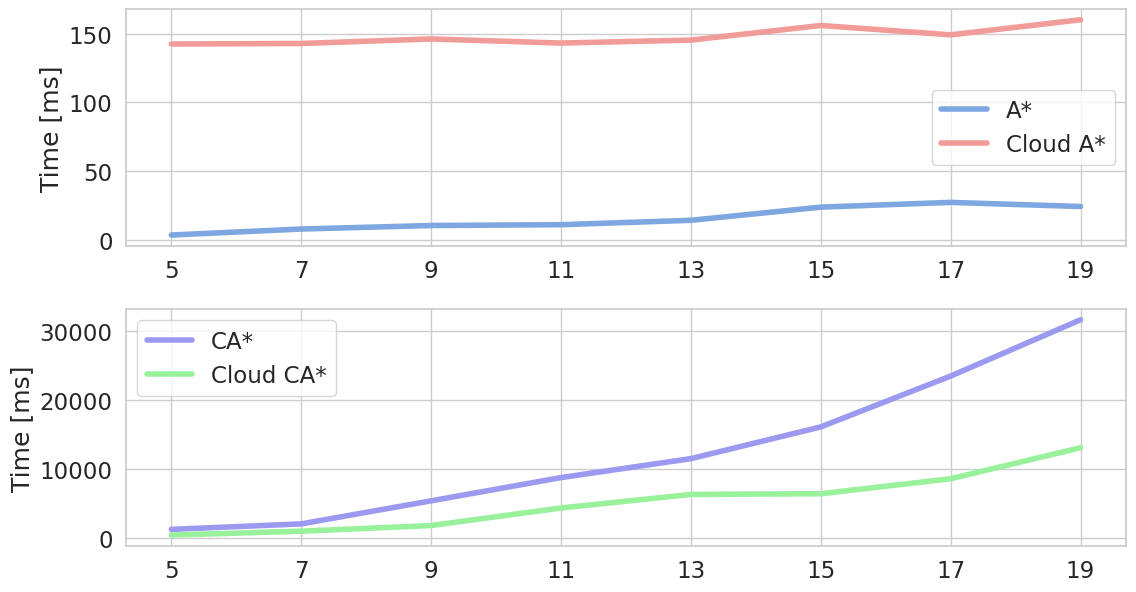
\includegraphics[width=0.75\textwidth]{pictures/on_prem_test_time.png}
    \caption{Test on on-prem setup}
    \label{fig:on_prem_test_time}
\end{figure}
\begin{figure}
    \centering
    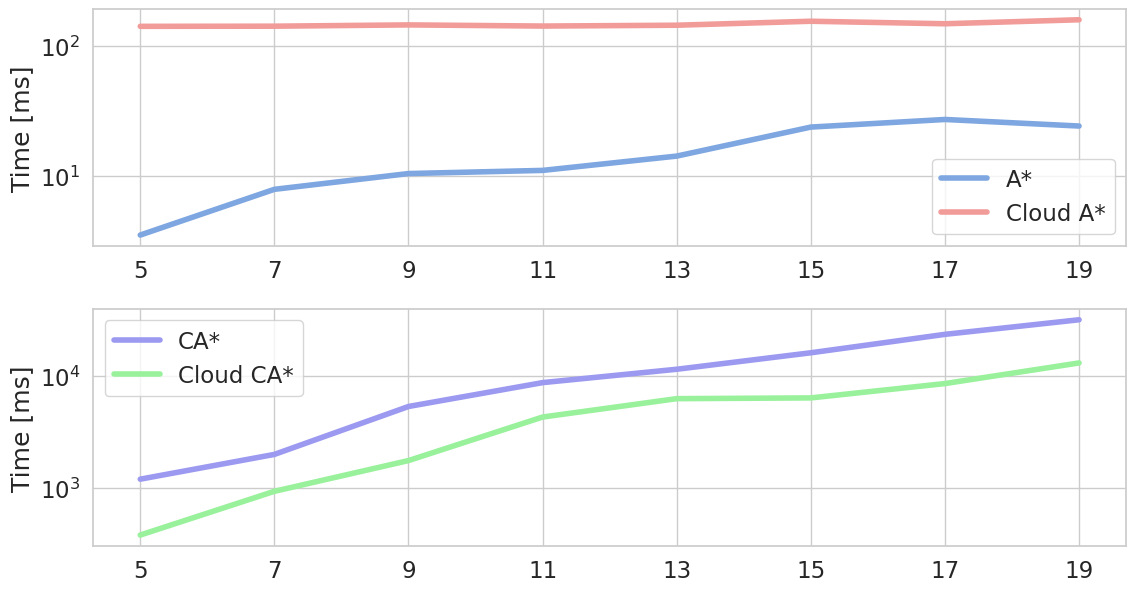
\includegraphics[width=0.75\textwidth]{pictures/on_prem_test_time_log.png}
    \caption{Test on on-prem setup in log scale}
    \label{fig:on_prem_test_time_log}
\end{figure}

Findings:
\begin{itemize}
    \item Non-collaborative algorithms are significantly faster than collaborative ones as they have lower time complexity. 
    \item Average time difference between A* and Cloud A* is around 150ms.
    \item Cloud A* has a higher deviation of the results than A*.
    \item CA* beats Cloud A* on the smallest map, on any other map Cloud CA* is performing better.
    \item Cloud CA* is around 10x faster on average than CA*.
\end{itemize}